\documentclass[11pt]{report}
\usepackage[utf8]{inputenc}	% Para caracteres en español
\usepackage{amsmath,amsthm,amsfonts,amssymb,amscd}
\usepackage{multirow,booktabs}
\usepackage[table]{xcolor}
\usepackage{fullpage}
\usepackage{lastpage}
\usepackage{enumitem}
\usepackage{fancyhdr}
\usepackage{mathrsfs}
\usepackage{wrapfig}
\usepackage{setspace}
\usepackage{hyperref}
\usepackage{calc}
\usepackage{multicol}
\usepackage{cancel}
\usepackage[retainorgcmds]{IEEEtrantools}
\usepackage[margin=3cm]{geometry}
\usepackage{amsmath}
\newlength{\tabcont}
\setlength{\parindent}{0.0in}
\setlength{\parskip}{0.05in}
\usepackage{empheq}
\usepackage{framed}
\usepackage[most]{tcolorbox}
\usepackage{xcolor}
\colorlet{shadecolor}{orange!15}
\parindent 0in
\parskip 12pt
\geometry{margin=1in, headsep=0.25in}
\theoremstyle{definition}
\usepackage{pdfpages}
\newtheorem{defn}{Definition}
\newtheorem{reg}{Rule}
\newtheorem{exer}{Exercise}
\newtheorem{note}{Note}
\usepackage{fancyhdr}\usepackage{xcolor}\usepackage{amsmath}\usepackage{amssymb}\pagestyle{fancy}\rhead{}
\newtheorem{theorem}{Theorem}[subsection]
\theoremstyle{definition}
\newtheorem{definition}[theorem]{Definiton}
\newtheorem{example}[theorem]{Example}
\newtheorem{corollary}[theorem]{Corollary}
\newtheorem{lemma}[theorem]{Lemma}
\title{Chapter 9 Review Notes}
\begin{document}
\thispagestyle{empty}
{\LARGE \bf CHE 260 Lecture Notes}\\
{\large Hei Shing Cheung}\\
Thermodynamics and Heat Transfer, Fall 2025 \hfill CHE260\\
\\
The up-to-date version of this document can be found at \url{https://github.com/HaysonC/skulenotes}\\

\begin{center}
    \textit{``If there is one word that describes this class it would be \textbf{energy}.''}
\end{center}
\chapter{Thermodynamics}
\begin{shaded}
    \section*{Systematic Approach to Problem Solving in Thermodynamics}
    You should adopt a systematic approach when tackling problems to avoid getting confused by a lot
    of information. The following steps are helpful:

    \begin{enumerate}
        \item \textbf{Find.} Read the problem and state what you are asked to find in your own words. This step
        may seem obvious, but it is surprising how often people misunderstand the question or
        miss essential information.
        \item \textbf{Known.} List all the information and properties provided, as well as information about properties that remain constant (e.g. the volume in a isochoric process or the temperature in an isothermal process).
        \item \textbf{Diagrams.} Draw a schematic diagram of the system. Mark the system boundary and decide whether the system is a control mass or volume. Show energy and mass transfers between the system and surroundings by arrows. Draw a process diagram if necessary.
        \item \textbf{Assumptions.} Decide how you are going to model the system. List all assumptions that you make.
        \item \textbf{Governing Equations.} Which conservation law are you going to apply? Depending on what you are trying to find, you may use principles of conservation of mass or energy. Write down the governing equations.
        \item \textbf{Properties.} List all property values that are not given in the problem statement. This includes information extracted from tables or other sources.
        \item \textbf{Solution.} Substitute known values of variables in the governing equations and solve them to find unknowns.
        \item \textbf{Answer.} State the answer and confirm that it is what was asked for.
        \item \textbf{Discussion.} Are your results reasonable? Can you draw any conclusions from them?
    \end{enumerate}


\end{shaded}
% ===================== PART 1: FOUNDATIONS =====================
\section{Foundations and Fundamental Concepts}
\begin{review}[Section overview]
Key ideas: energy and entropy as fundamental concepts; systems, states, and properties. Tips: always sketch system boundary and list knowns/assumptions. Units: keep Joule and Watt consistent (W = J/s).
\end{review}
\begin{definition}[Energy]
    You should have learned that energy is the ability to do work.
\end{definition}


\begin{definition}[Work]
    You also learned that work is the transfer of energy.
\end{definition}

We have a problem. The above two definitions are in terms of each other. This touches on the theory of fundamental concepts:

\paragraph{Fundamental Concepts} For example, the following are fundamental concepts in physics:
\begin{itemize}
    \item Time
    \item \textbf{Mass} Interestingly, we don't measure mass directly; instead, we measure weight, which is the force exerted by gravity on an object, and from that we deduce mass.
    \item Space
\end{itemize}
In this course, we are going to explore two:
\begin{itemize}
    \item \textbf{Energy} Energy is pretty familiar to us. 
    \item \textbf{Entropy} Entropy is what gives students the most trouble; you can't show someone a picture of entropy, it is abstract.
\end{itemize}

These fundamental concepts are in arbitrary units and form the foundation `axioms' in science. We first build intuitive physical meaning (ability to lift, cause motion, create change) before formal laws.

\subsection{Mechanical Intuition for Energy Forms}
\paragraph{Energy} An understanding of energy is its ability to \textbf{lift weights}. This is a way we could test if there is energy.
\begin{example}[Potential Energy]
    A 1 kg mass lifted 1 meter has a potential energy of about 10 J. Imagine that it is attached to a balance, with a small mass on the other side, then, it is able to lift that weight.
\end{example}

\begin{example}[Kinetic Energy]
    Given a flying ball that hits a lever with a mass rested on it, given the appropriate angle, the ball can transfer its kinetic energy to the mass, causing it to lift.
\end{example}

\begin{example}[Heat]
    Given a gas in a container, if we heat the gas, it expands and lifts objects on top of it.
\end{example}
\begin{shaded}
\begin{example}[Newcomen Engine]
    The above example is actually a simplified representation of how the Newcomen engine operates. In the Newcomen engine, steam is used to create a vacuum that lifts a piston, demonstrating the conversion of thermal energy into mechanical work.
\end{example}
\end{shaded}
\begin{figure}[h!]
    \centering
    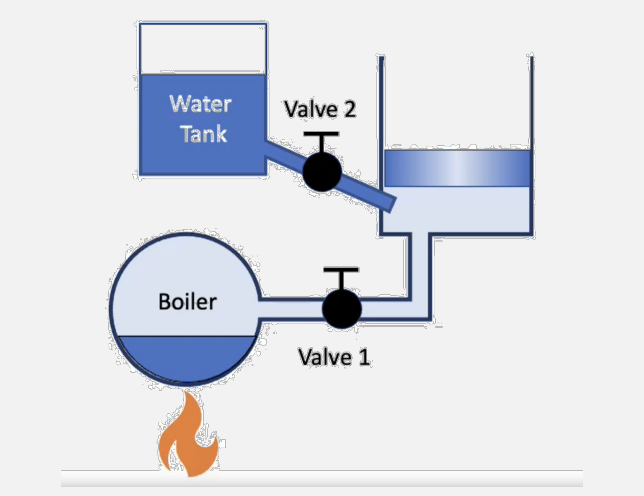
\includegraphics[width=0.5\textwidth]{newcomen_engine.png}
    \caption{A Newcomen Engine}
\end{figure}
When Valve 1 opens, steam fills the chamber and lifts up the piston. When Valve 2 opens (with valve 1 closes),
water gets sprayed, evaporates, and condenses, causing the piston to lower.

However, the Newcomen engine is not the most efficient steam engine, most heat is lost in the heating and cooling process. Solution? A external condenser was added to improve efficiency by cooling the steam and creating a vacuum, allowing the piston to be pulled down more effectively. This is the \textbf{Watt Engine}.

\paragraph{Steam Cycle (Preview)} The steam cycle is a thermodynamic cycle that converts heat energy into mechanical work. It consists of four main processes (we will formalize cycles later under engines): 
\begin{enumerate}
    \item \textbf{Heating} - The working fluid (steam) is heated in the boiler, converting water into steam and increasing its energy.
    \item \textbf{Expansion} - The high-pressure steam expands in the piston, doing work on the piston and converting thermal energy into mechanical work.
    \item \textbf{Cooling} - The steam is cooled in the condenser, releasing heat to the surroundings and condensing back into water.
    \item \textbf{Compression} - The water is pumped back into the boiler, completing the cycle.
\end{enumerate}

\begin{figure}[h!]
    \centering
    \begin{tikzpicture}
        \node (boiler) [rectangle, draw] {1. Boiler};
        \node (turbine) [rectangle, draw, right=of boiler] {2. Turbine};
        \node (condenser) [rectangle, draw, below=of turbine] {3. Condenser};
        \node (pump) [rectangle, draw, below=of boiler] {4. Pump};

        \draw[->] (boiler) -- (turbine);
        \draw[->] (turbine) -- (condenser);
        \draw[->] (condenser) -- (pump);
        \draw[->] (pump) -- (boiler);
    \end{tikzpicture}
    \caption{Steam Cycle Diagram}
\end{figure}

\begin{definition}[Heat Engine]
    A heat engine is a device that converts thermal energy into mechanical work. It operates by taking in heat from a high-temperature source, performing work using that heat, and then releasing some waste heat to a low-temperature sink. The steam engine is a classical instance of a heat engine.
\end{definition}
\begin{figure}[h!]
    \centering
    \begin{tikzpicture}
        \node (Engine) [circle, draw] {Heat Engine};
        \node (Source) [rectangle, draw, left=of Engine] {High-Temp Source ($Q_H$)};
        \node (Sink) [rectangle, draw, right=of Engine] {Low-Temp Sink ($Q_C$)};
        \draw[->] (Source) -- (Engine);
        \draw[->] (Engine) -- (Sink);  

        \node (Work) [rectangle, draw, below=of Engine] {Work Output ($W$)};
        \draw[->] (Engine) -- (Work);
    \end{tikzpicture}
    \caption{A Heat Engine}
\end{figure}

\paragraph{Efficiency of a Heat Engine} The efficiency of a heat engine is defined as the ratio of the work output to the heat input:
\keyeq{\eta = \frac{W}{Q_H}}

Obviously, the best engine is when $\eta$ is maximized ($W$ is maximized, and $Q_H$ is minimized). For example, a Newcomen engine has a low efficiency ($\eta \approx 0.34\%$), while a classic watt engine has a higher efficiency ($\eta \approx 4\%$). The modern powerplant is optimized such that it has $\eta \approx 30\%$.

This begs the question, can we create a heat engine with 100\% efficiency (i.e., $Q_C = 0$)? The answer is no, due to the second law of thermodynamics [Sadi Carnot (1830)]. For now, consider the wasted energy $Q_c$. 

\paragraph{Irreversibility and Spontaneity} The process of losing heat is spontaneous and irreversible. Once heat is lost to the cooler surroundings, it cannot be completely recovered and converted back into work, however, the process of bringing heat from a cooler body to a hotter body is non-spontaneous and requires external work (e.g., a refrigerator). These give rise to the concept of irreversibility in thermodynamic processes, from the laws of thermodynamics.

% ===================== PART 2: LAWS OF THERMODYNAMICS (PREVIEW) =====================
\section{Preview of Thermodynamic Laws and Directionality}
\begin{review}[Section overview]
Most-used relations: \noteeq{W = Q_H - Q_C}, sign convention (to system positive), and “heat flows hot→cold.” Pitfall: mixing absolute temperature (K) with Celsius.
\end{review}
The first intuitive principle (later formalized) is conservation of energy in transformations between forms:
\begin{definition}[First Law of Thermodynamics] \label{def:firstlaw}
    The first law of thermodynamics states that energy cannot be created or destroyed, only transformed from one form to another. In the context of a heat engine, this means that the work output ($W$) is equal to the heat input ($Q_H$) minus the heat rejected ($Q_C$):
    \keyeq{ W = Q_H - Q_C }
\end{definition}
The second law formalizes directionality: heat does not spontaneously flow from cold to hot. This introduces \emph{entropy} as a bookkeeping tool for irreversibility. (A rigorous treatment of entropy will follow after we develop state / property concepts.)

\begin{definition}[Second Law of Thermodynamics]
    The second law of thermodynamics states that the total entropy of an isolated system can never decrease over time. We consdier entropy as:
    \numeq{ S = \frac{Q}{T} }
    In the above example, we can see that entropy increases as heat is transferred from the hot reservoir to the cold reservoir:

    \keyeq{ \Delta S = \frac{Q_C}{T_C} - \frac{Q_H}{T_H} > 0 }

    Since $Q_C = Q_H$ in a closed system and $T_H > T_C$, we have $\Delta S > 0$.
\end{definition}



% ===================== PART 3: SYSTEM DESCRIPTORS =====================
\section{Systems, States, and Properties}
\begin{review}[Section overview]
System types: closed (no mass), open/control volume (mass+energy), isolated (no mass or energy). Property vs path-dependent: properties (T, P, V, U, m) vs. transfers (Q, W). Pitfall: use \(\delta W, \delta Q\) for path differentials.
\end{review}
\begin{definition}[System]
    Any piece of matter or a region of space.
\end{definition}

\begin{definition}[Boundary]
    The boundary is the surface that separates the system from its surroundings. It can be real or imaginary, fixed or movable, and can allow or prevent the transfer of mass and energy.
\end{definition}

\textbf{Types of Systems} There are three main types of systems: closed, open, and isolated. Defined as the following:
\begin{definition}[Closed System/Control Mass]
    A closed system is one where mass cannot cross the boundary, but energy can. An example of a closed system is a sealed container of liquid, or a bag of gas, where we can do work on it.
\end{definition}
\begin{definition}[Open System/Control Volume]
    An open system is one where both mass and energy can cross the boundary. An example of an open system is a flowing pipe, or a car engine, where mass (water, air) and energy (heat, work) can enter and leave the system.
\end{definition}
\begin{definition}[Isolated System]
    An isolated system is one where neither mass nor energy can cross the boundary. An example of an isolated system is a thermos bottle that is perfectly insulated from its surroundings.
\end{definition}
\begin{definition}[Property]
    A property is any attribute of a system that can be measured without knowing the history of the system. \\
    (Example) Position, Temperature, Mass, Energy \\
    (Non-example) Work, Transfer of energy (heat), Mass outside the system (denote $\delta m$)
    \numeq{ W = \int \! \delta W \quad (\text{depends on path}) }
    Hence, to remind ourselves, we denote infinitesimal work as $\delta W$ instead of $dW$. Then, we can compute the work done by the force field $\textbf{F}$ along a curve $C$ as:
    \begin{equation}
        \delta W = \int_C \textbf{F} \cdot ds
    \end{equation}
\end{definition}
\begin{shaded}
Here's a quick refresher on line integrals and basic math:
\begin{example}[Computing work]
    \textit{The force acting on a 5 kg object varies with time as F = $(50 + 10t)\,N$, where t is the time in seconds. If the body starts from rest, how much work is done on it in 10 s?}

    The object is travelling for a straight line, so we can simply parametrize the curve as $ds = v dt = r' dt$. We can compute the velocity $v$ by integrating the acceleration $a = F/m$. Firstly the work is given by:
    $$
        W = \int_{C} F \cdot ds = \int_0^{10} F \cdot v dt
    $$
    Since they are in the same direction, we can treat them as scalars. Now, we compute $v$:
    $$
        v = \int_0^t a dt = \int_0^t \frac{F}{m} dt = \int_0^t \frac{50 + 10t}{5} dt = 10t + t^2 + (\text{$C$ = 0 $\because$ object starts from rest})
    $$
    Hence, we have:
    $$
        W = \int_0^{10} (50 + 10t)(10t + t^2) dt = 100\,000 \text{ J}
    $$
\end{example}

\end{shaded}
\paragraph{Intensive and Extensive Properties} Properties can be classified into two categories: intensive and extensive.
\begin{definition}[Extensive Property]
    An extensive property is one that depends on the size or extent of the system. \\
    (Example) Mass, Volume, Energy
\end{definition}    
\begin{definition}[Intensive Property]
    An intensive property is one that does not depend on the size or extent of the system. \\ 
    (Example) Temperature, Pressure, Density 

    We can convert any extensive property to an intensive property by dividing it by mass or volume. For example, specific volume $v$ or specific energy $u$:
    $$
        v = \frac{V}{m}, \quad u = \frac{U}{m}
    $$
\end{definition}

\begin{definition}[State]
    The state of a system is defined by its properties at a specific moment in time. A state is a condition of the system that can be described by a set of properties. For example, the state of an ideal gas can be described by its pressure, volume, and temperature.
    
\end{definition}

\begin{definition}[Steady State]
    A system is in steady state if its properties do not change with time. In other words, the system is in a state of equilibrium, and there are no net changes in mass or energy within the system. \\
    (Example) An overflowing bucket of water, in which case the system is unchanging but interacting with its surroundings.
\end{definition}

\begin{definition}[Equilibrium]
    An \textbf{ISOLATED} system is in equilibrium if its properties are uniform throughout the system and do not change with time (constant). \\
    (Example) A gas in a closed container that has been left undisturbed for a long time.
\end{definition}
\begin{example}
    Consider a gas in a cylinder with a movable piston. If the piston is held in place, the gas is in a steady state, as its properties (pressure, volume, temperature) do not change with time. However, if the piston is allowed to move, the gas will expand or compress, and its properties will change with time, indicating that it is not in a steady state. 
\end{example}
\begin{definition}[Process]
    A process is a transformation from one state to another. A process can be described by the path taken by the system in the property space. For example, a gas can undergo a process of compression or expansion, which changes its pressure, volume, and temperature.
\end{definition}

% ===================== PART 4: IDEAL GAS MODEL =====================
\section{Ideal Gas Model and Molecular Basis}
\begin{review}[Section overview]
Ideal gas: \noteeq{PV = n R_u T = m R T}. Useful processes: isothermal (\noteeq{PV=\text{const}}), adiabatic reversible (\noteeq{PV^\gamma=\text{const}}, \noteeq{TV^{\gamma-1}=\text{const}}). Pitfalls: use absolute T (K); check units of R.
\end{review}
\begin{definition}[Quasi-Equilibrium Process (Reversible Path)]
    A quasi-equilibrium process is a process that occurs slowly enough that the system remains in a state of equilibrium at all times. In other words, the properties of the system change so (infinitely) slowly that they can be considered constant during the process. In this case, this path is reversible. \\
    (Example) A gas in a cylinder with a movable piston that is compressed or expanded very slowly, allowing the gas to remain in equilibrium throughout the process.
\end{definition}

\begin{definition}[Real Process (Irreversible Path)]
    A real process is a process that occurs at a finite rate, and the system may not remain in a state of equilibrium at all times. In other words, the properties of the system may change rapidly during the process, and the system may not be able to adjust to these changes quickly enough to maintain equilibrium. In this case, this path is irreversible. \\
    (Example) A gas in a cylinder with a movable piston that is compressed or expanded quickly, causing the gas to deviate from equilibrium during the process. In that process, the work done is more than that of a quasi-equilibrium process.
\end{definition}

\begin{shaded}
\paragraph{Motivation} We care about this because this is the process in which we ignite an engine, allowing gas to expand rapidly, pushing the piston down and doing work.
\end{shaded}

\begin{definition}[Ideal Gas Model]
    Consider an isolated system with molecules that:
    \begin{itemize}
        \item Have negligible volume compared to the volume of the container. (point mass)
        \item Do not interact with each other except during elastic collisions.
        \item Are in constant random motion without spin or vibration.
    \end{itemize}
    The best example of this is a noble gas (e.g., helium, neon, argon). Since they are inert and monoatomic. For all we care about in this course all gas are ideal unless:
    \begin{itemize}
        \item They are at very high pressure (Condier more then 1 atm).
        \item They are at very low temperature (Consider close to 0 K).
    \end{itemize}
\end{definition}

Such a system is called an ideal gas. The macroscopic observation of pressure is the average force per unit area exerted by the gas molecules colliding with the walls of the container, so if we increase the number of molecules or decrease the volume, the pressure increases proportionally, this is Boyle's law:

\begin{definition}[Boyle's Law]
    For a given amount of gas at constant temperature, the pressure of the gas is inversely proportional to its volume:
    \begin{equation}
        P \propto \frac{1}{V} \quad \Rightarrow \quad PV = \text{constant}
    \end{equation}
    where $N$ is the number of molecules. We can proof the $PV$ inverse relationship a momentum conservation argument. Consider linear path with lenght $L$, since collisions are elastic, the change in momentum for each collision is $\Delta p = 2mv_x$. The time between collisions is $\Delta t = \frac{2L}{v_x}$, so the force exerted on the wall is:
    $$
        F = \frac{\Delta p}{\Delta t} = \frac{2mv_x}{\frac{2L}{v_x}} = \frac{mv_x^2}{L}
    $$
    The pressure is then given by:
    $$
        P = \frac{F}{A} = \frac{mv_x^2}{AL} = \frac{mv_x^2}{V}
    $$
    Thus, we have $PV \propto mv_x^2$. Now, define the RMS velocity as $v_{rms} = \sqrt{\frac{1}{N} \sum_{i=1}^N v_i^2}$, and consider random motion, we have $\overline{v_x^2} = \overline{v_y^2} = \overline{v_z^2} = \frac{1}{3} v_{rms}^2$. Hence, we have:
    $$
        PV \propto Nm \overline{v_x^2} = \frac{1}{3} Nm v_{rms}^2
    $$
    where $Nm$ is the total mass of the gas. Then, we complete the arguement of the gas moving in all direction.
\end{definition}

\begin{example}[Boyle's Law]
    Consider a gas in a cylinder with a movable piston. If we compress the gas by pushing the piston down, the volume of the gas decreases, and the pressure increases. This relationship is described by Boyle's law, which states that for a given amount of gas at constant temperature, the pressure of the gas is inversely proportional to its volume:
\end{example}

We can also observe that increasing the temperature increases the average kinetic energy of the molecules, which increases the frequency and force of collisions with the walls of the container, leading to an increase in pressure, this is Charles's law:
\begin{definition}[Charles's Law, Total Internal Energy]
    For a given amount of gas at constant volume, the pressure of the gas is directly proportional to its absolute temperature:
    \begin{equation}
        P \propto T
    \end{equation}
    And the total internal energy of an ideal gas is the sum of the kinetic energies of all the gas molecules, which is also directly proportional to its absolute temperature:
    \begin{equation}
        U = \frac{3}{2} N k_B T = \frac{3}{2} n R_u T
    \end{equation}
    $U$ is a extensive property, so it is proportional to the number of molecules $N$ (or moles $n$). The intensive property is the specific internal energy:
    \begin{equation}
        u = \frac{U}{m} = \frac{3}{2} \frac{R_u}{M} T = \frac{3}{2} R T
    \end{equation}
    where $M$ is the molar mass of the gas, and
    \begin{equation}
        R = \frac{R_u}{M}
    \end{equation}
    is the specific gas constant.

    This is a consequence of the kinetic theory of gases, which model temperature as the average kinetic energy of the gas molecules, so we have:
    \begin{align*}
        \frac{1}{2} mv_{rms}^2 &= \frac{3}{2} R_u T \\
        \intertext{Dividing by $N_A$ (Avogadro's number), and define the boltzmann constant $k_B = \frac{R_u}{N_A}$, we have:}
        \frac{1}{2} m_e v_{rms}^2 &= \frac{3}{2} k_B T 
        \intertext{We multiply both sides by $N$ (number of molecules), and substitute into the previous equation, we have:}
        \frac{1}{2} m_e v_{rms}^2 N &= \frac{3}{2} k_B T N \\
    \end{align*}
    The above is the internal energy of the gas. Thus, we can deduce the following Ideal Gas Law, which matches macroscopic observations:
\end{definition}

\begin{definition}[Ideal Gas Law]
    Consider the combination of Boyle's and Charles's law, we have the ideal gas law:
    \begin{equation}
        PV = nR_uT = mRT
    \end{equation}
    where $R_u = 8.314\, \text{J/(mol K)}$ (or, equivalently, $R_u = 8 \times 10^3 \, \text{J/(kmol K)}$) is the universal gas constant, and $n$ is the number of moles of gas. $R = \frac{R_u}{M}$ is the specific gas constant, where $M$ is the molar mass of the gas.
\end{definition}

\begin{example}
    \textit{A spherical balloon with $d = 6\, m$ is filled with helium gas at $P = 200$ kPa and $T = 20^\circ C$. Calculate the mass and number of moles of helium in the balloon. (Assume ideal gas behavior).}

    We can use the ideal gas law to solve this problem. First, we need to calculate the volume of the balloon:
    $$        
    V = \frac{4}{3} \pi r^3 = \frac{4}{3} \pi (3)^3 = 113.1\, \text{m}^3
    $$
    Next, we can use the ideal gas law to calculate the number of moles of helium in the balloon:
    $$
        n = \frac{PV}{R_uT} = \frac{200 \times 10^3 \times 113.1}{8.314 \times (20 + 273)} = 9\,280\, \text{mol}
    $$
    Finally, we can calculate the mass of helium in the balloon using the molar mass of helium ($M = 4\, \text{g/mol}$):
    $$
        m = nM = 9\,280 \times 4  = 37\,120\, \text{g} = 37.12\, \text{kg}
    $$
\end{example}

\begin{example}[Adiabatic Compression]
    Consider an ideal gas undergoing adiabatic compression\footnote{This differs from \textbf{isothermal} compression, where the temperature remains constant.}. 
    Since no heat is exchanged with the surroundings ($Q=0$), the work done on the gas increases its internal energy, which raises the temperature. 
    Using the adiabatic relations,
    $$
        P V^{\gamma} = \text{constant}, 
        \quad T V^{\gamma - 1} = \text{constant},
    $$
    we see that a decrease in $V$ leads to an increase in both $P$ and $T$.
\end{example}

\begin{example}[Isothermal Expansion]
    Consider an ideal gas undergoing isothermal expansion\footnote{This differs from \textbf{adiabatic} expansion, where no heat is exchanged.}. 
    Since the temperature remains constant ($\Delta T = 0$), the internal energy of the gas does not change ($\Delta U = 0$). 
    The work done by the gas during expansion is equal to the heat absorbed from the surroundings ($Q = W$). 
    Using the ideal gas law, we can see that as $V$ increases, $P$ decreases, while $T$ remains constant.
    
\end{example}

\paragraph{Note} For all ideal gas processes, the internal energy $U$ depends only on temperature $T$, not on pressure $P$ or volume $V$. This is a key property of ideal gases and simplifies the analysis of thermodynamic processes involving them.

\begin{definition}[Change in Internal Energy]
    The change in internal energy of an ideal gas can be calculated using the specific heat capacity at constant volume ($c_v$):
    \begin{equation}
        \Delta U = \frac{3}{2} mk_B \Delta T = m c_v \Delta T
    \end{equation}
    where $c_v$ [J kg$^{-1}$ K$^{-1}$] is the specific heat capacity at constant volume. For a monoatomic ideal gas, we have:
    \begin{equation}
        c_v = \frac{3}{2} R
    \end{equation}
    where $R$ is the specific gas constant.
\end{definition}

\begin{example}
    \textit{How much energy is required to heat 10kg of air with 20$^\circ$C at 1 bar to 120$^\circ$ at constant volume? What is the final pressure? (Assume ideal gas behavior, and $c_{v, \text{air}} = 0.717$ kJ/kg K)}

    Consider the change of internal energy:
    $$
        \Delta U = m c_v \Delta T = 10 \times 100 \times c_{v, \text{air}} = 1\,000 \times 0.717 = 717\, \text{kJ}
    $$

    Now consider the change of pressure, we first isolate for the control:
    $$
        \frac{mR}{V} = \frac{P}{T}
    $$
    So we can compute the final pressure:
    $$
        \frac{P_1}{T_1} = \frac{P_2}{T_2} \Rightarrow P_2 = P_1 \frac{T_2}{T_1} = 1 \times \frac{393}{293} = 1.34\, \text{bar}
    $$
\end{example}

% ===================== PART 5: FIRST LAW FORMAL DEVELOPMENT =====================
\section{First Law of Thermodynamics (Formal Development)}
\begin{review}[Section overview]
Closed system: \noteeq{\Delta U=Q-W}. Control volume steady state (single-in/out): \noteeq{\dot W_{shaft}=\dot m(h_1-h_2)+\dot m(\tfrac{V_1^2-V_2^2}{2}+g(z_1-z_2)) - (\dot Q_1-\dot Q_2)}. Sign convention: work out of system positive.
\end{review}
\begin{shaded}
\paragraph{Motivation} We want to understand how energy is conserved in a system, and how energy is transferred between a system and its surroundings. This is important for understanding how engines work, how to design efficient systems, and how to analyze thermodynamic processes.
\end{shaded}  
The same definition as before \ref{def:firstlaw}.

\begin{definition}[First Law of Thermodynamics for a Closed or Isolated System]
    For a closed system, the energy balance can be expressed as:
    \begin{equation}
        \Delta E_{in} - \Delta E_{out} = \Delta E_{system}
    \end{equation}
    where $\Delta E_{in}$ is the energy entering the system, $\Delta E_{out}$ is the energy leaving the system, and $\Delta E_{system}$ is the change in energy of the system. The total energy of the system can be expressed as:
    \begin{equation}
        E_{system} = U + KE + PE
    \end{equation}
    where $U$ is the internal energy, $KE$ is the kinetic energy, and $PE$ is the potential energy.
\end{definition}

\paragraph{Sign Convention} Relative to a system, we adopt the following sign convention:
\begin{itemize}
    \item Energy transfer to the system is positive.
    \item Energy transfer from the system is negative.
\end{itemize}

\begin{definition}[Energy Transfer from a System]
    The energy transfer from a system can occur in two ways: heat transfer ($Q$) and work transfer ($W$). The first law of thermodynamics can be expressed as:
    \begin{equation}
        dE = \delta Q + \delta W
    \end{equation}
\end{definition}

Dividing by $dt$, we have the rate form of the first law:
\begin{definition}[Rate Equation of the First Law of Thermodynamics]
    \begin{equation}
        \frac{dE}{dt} = \dot{Q} + \dot{W}
    \end{equation}
    where $\dot{Q}$ is the rate of heat transfer, and $\dot{W}$ is the rate of work transfer.
\end{definition}

% ===================== PART 6: WORK AND ENERGY MODES =====================
\section{Work and Energy Transfer Modes}
\begin{review}[Section overview]
Boundary work for quasi-equilibrium: \noteeq{W=\int P\,dV}. Useful cases: isobaric \noteeq{W=P\Delta V}, isothermal ideal gas \noteeq{W=nRT\ln(V_2/V_1)}. Flow work is included in enthalpy: \noteeq{h=u+Pv}.
\end{review}
\begin{definition}[Boundry Work]
    Force acts on the boundries of a systems and deformes them. \\
    (Example) Expansion and compression of a gas 

    Assuming for a Quaso-equilibrium process, and no friction, we can compute the boundary work as:
    \begin{equation}
        \delta W = F dx  = P A dx = - P dV
    \end{equation}
    where $P$ is the pressure of the gas, $A$ is the area of the piston, and $dx$ is the displacement of the piston. The negative sign is because when the gas expands, it does work on the surroundings, so the work done by the system is negative. Also, we can consider the total work by:
    \begin{equation}
        w_{12} = -\int_{V_1}^{V_2} P dV
    \end{equation}
    \text{Note} Connecting that to the $PV$ diagram, the work done by the system is the area under the curve in the $PV$ diagram:

\begin{figure}[h!]
    \centering
    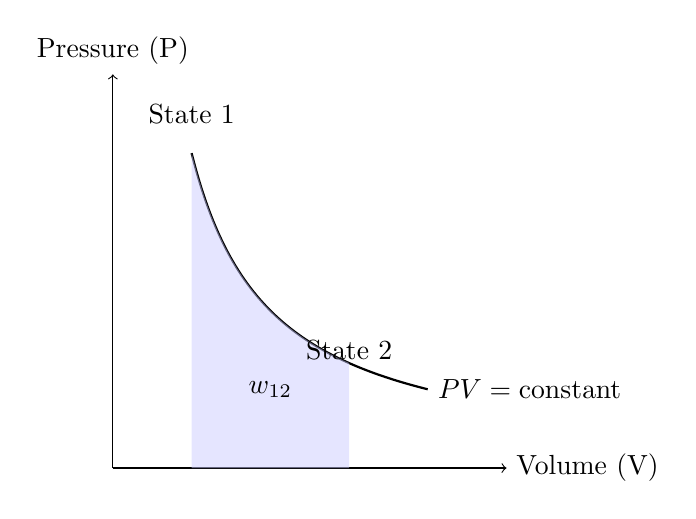
\begin{tikzpicture}
        \draw[->] (0,0) -- (5,0) node[right] {Volume (V)};
        \draw[->] (0,0) -- (0,5) node[above] {Pressure (P)};
        \draw[thick, domain=1:4, samples=100] plot (\x, {4/\x}) node[right] {$P V = \text{constant}$};
        \fill[blue!20, opacity=0.5] (1,4) -- plot[domain=1:3] (\x, {4/\x}) -- (3, 0) -- (1, 0) -- cycle;
        \node at (2,1) {$w_{12}$};
        \node at (1,4.5) {State 1};
        \node at (3,1.5) {State 2};
    \end{tikzpicture}
    \caption{Work done by the system during expansion from State 1 to State 2 is the area under the curve in the $PV$ diagram.}
\end{figure}

\end{definition}
\newpage
\begin{example}[Isochoric Process]
    Consider a gas in a cylinder with a fixed piston. If we heat the gas, its temperature and pressure increase, but its volume remains constant. In this case, there is no boundary work done by the system, as the volume does not change ($dV = 0$). However, there may be other forms of work done on or by the system, such as electrical work if the gas is heated using an electric heater. We can demosrate by the below diagram:
    \begin{figure}[h!]
        \centering
        \begin{tikzpicture}
            \draw[->] (0,0) -- (5,0) node[right] {Volume (V)};
            \draw[->] (0,0) -- (0,5) node[above] {Pressure (P)};
            \draw[thick] (2,0.5) -- (2,4) node[above] {};    
            \node at (2.25,2) {$w_{12} = 0$};
            \node at (2,4.5) {State 2};
            \node at (2,0.5) {State 1};
        \end{tikzpicture}
        \caption{Isochoric Process in a $PV$ Diagram}
    \end{figure}
    
\end{example}

\begin{example}[Isobaric Process]
    Consider a gas in a cylinder with a movable piston with mass $m$ on top. If we heat the gas, its temperature and volume increase, while its pressure remains constant (equal to the atmospheric pressure plus the pressure exerted by the mass on top of the piston). In this case, there is boundary work done by the system as the volume changes ($dV \neq 0$). The work done by the system can be calculated using the formula:
    \begin{equation}
        w_{12} = -\int_{V_1}^{V_2} P dV = -P (V_2 - V_1)
    \end{equation}
    where $P$ is the constant pressure of the gas, and $V_1$ and $V_2$ are the initial and final volumes of the gas, respectively. We can demonstrate by the below diagram:
    \begin{figure}[h!]
        \centering
        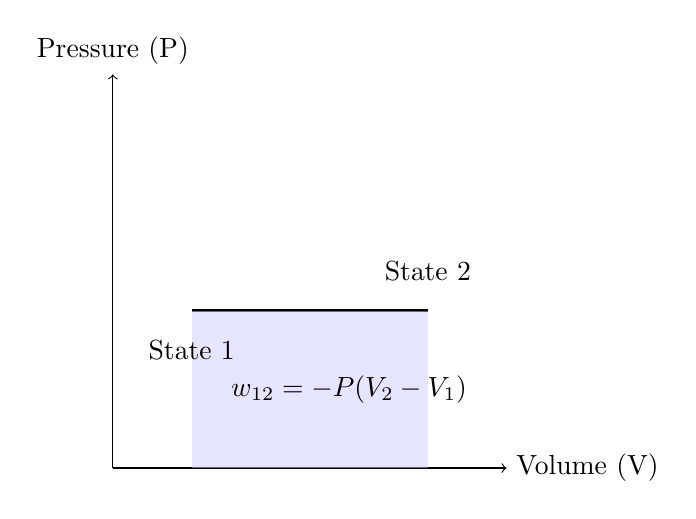
\begin{tikzpicture}
            \draw[->] (0,0) -- (5,0) node[right] {Volume (V)};
            \draw[->] (0,0) -- (0,5) node[above] {Pressure (P)};
            \draw[thick] (1,2) -- (4,2) node[right] {};    
            \fill[blue!20, opacity=0.5] (1,0) -- (4,0) -- (4,2) -- (1,2) -- cycle;
            \node at (3,1) {$w_{12} = -P (V_2 - V_1)$};
            \node at (4,2.5) {State 2};
            \node at (1,1.5) {State 1};
        \end{tikzpicture}
        \caption{Isobaric Process in a $PV$ Diagram}
    \end{figure}
\end{example}

\begin{example}[Isothermal Process]
    Consider a gas in a cylinder with a movable piston. If we compress the gas very slowly while keeping it in contact with a thermal reservoir, its temperature remains constant (isothermal process). In this case, there is boundary work done by the system as the volume changes ($dV \neq 0$). The work done by the system can be calculated using the formula:
    \begin{equation}
        w_{12} = -\int_{V_1}^{V_2} P dV = -nR_u T \ln\left(\frac{V_2}{V_1}\right)
    \end{equation}
    where $n$ is the number of moles of gas, $R_u$ is the universal gas constant, $T$ is the constant temperature of the gas, and $V_1$ and $V_2$ are the initial and final volumes of the gas, respectively. We can demonstrate by the below diagram:
    \begin{figure}[h!]
        \centering
        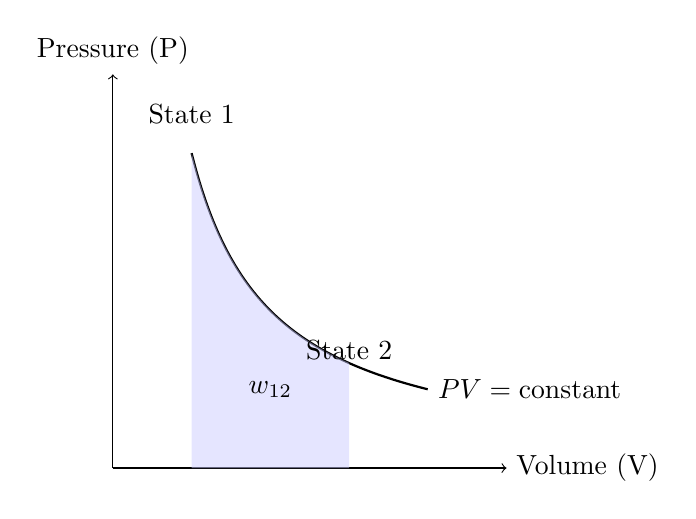
\begin{tikzpicture}
            \draw[->] (0,0) -- (5,0) node[right] {Volume (V)};
            \draw[->] (0,0) -- (0,5) node[above] {Pressure (P)};
            \draw[thick, domain=1:4, samples=100] plot (\x, {4/\x}) node[right] {$P V = \text{constant}$};
            \fill[blue!20, opacity=0.5] (1,4) -- plot[domain=1:3] (\x, {4/\x}) -- (3, 0) -- (1, 0) -- cycle;
            \node at (2,1) {$w_{12}$};
            \node at (1,4.5) {State 1};
            \node at (3,1.5) {State 2};
        \end{tikzpicture}
        \caption{Isothermal Process in a $PV$ Diagram}
    \end{figure}

    We can use the above equation to calculate the work done by the gas during the isothermal compression process.
    
\end{example}

\paragraph{General Polytropic Representation} In general, we can fit a curve in the $PV$ diagram using the polytropic process equation:
\begin{equation}
    P V^n = \text{constant}
\end{equation}
where $n$ is the polytropic index. Different values of $n$ correspond to different specific types of processes:
\begin{itemize}
    \item $n = 0$: Isobaric process (constant pressure)
    \item $n = 1$: Isothermal process (constant temperature)
    \item $n = \gamma$: Adiabatic process (no heat transfer, where $\gamma = \frac{c_p}{c_v}$ is the heat capacity ratio)
    \item $n \to \infty$: Isochoric process (constant volume)
\end{itemize}
We can compute the work done by the system during a polytropic process as:
\begin{equation}
    w_{12} = -\int_{V_1}^{V_2} P dV = \frac{P_2 V_2 - P_1 V_1}{n - 1} \quad (n \neq 1)
\end{equation}

\begin{definition}[Flow Work]
    Flow work is the work required to push mass into or out of a control volume. It is given by:
    \begin{equation}
        W_{flow} = \frac{PB}{m} = Pv
    \end{equation}
    where $P$ is the pressure, $B$ is the volume flow rate, and $m$ is the mass flow rate. $v$ is the specific volume (volume per unit mass).
    
    \textbf{Energy flowing a system per unit mass of a fluid} is called \textbf{flow energy} or \textbf{flow work}. It is the energy required to push mass into or out of a control volume. The flow work per unit mass is given by enthalpy, which we will define next.
\end{definition}


\begin{definition}[Enthalpy]
    Enthalpy is a thermodynamic property that represents the total energy of a system, including both its internal energy and the energy associated with its pressure and volume. It is defined as:
    \begin{equation}
        H = U + PV
    \end{equation}
    where $H$ is the enthalpy, $U$ is the internal energy, $P$ is the pressure, and $V$ is the volume. Enthalpy is an extensive property, so we can define the specific enthalpy as:
    \begin{equation}
        h = u + Pv
    \end{equation}
    where $h$ is the specific enthalpy, $u$ is the specific internal energy, and $v$ is the specific volume.
    
\end{definition}

\begin{example}[Constant Pressure Porcess]
    Consider a gas in a cylinder with a movable piston. If we heat the gas at constant pressure, we would haveL
    $$
        P_{\text{gas}} = P_{\text{atm}}
    $$
    The work done by the gas during expansion is given by:
    $$
        w_{12} = -\int_{V_1}^{V_2} P dV = -P (V_2 - V_1)
    $$
    The energy balance for the system can be expressed as:
    $$
        Q_{\text{in}} - W_{\text{out}} = \Delta U_{\text{system}}
    $$
    where $Q_{\text{in}}$ is the heat added to the system, $W_{\text{out}}$ is the work done by the system, and $\Delta U_{\text{system}}$ is the change in internal energy of the system. Rearranging, we have:
    $$
        Q_{\text{in}} = (U_2 - U_1) + (P_2 V_2 - P_1 V_1) = (U_2 + P_2 V_2) - (U_1 + P_1 V_1) = H_2 - H_1
    $$
\end{example}

\begin{theorem}[Enthalpy Change in a Constant Pressure Process]
    For a constant pressure process, the heat added to the system is equal to the change in enthalpy of the system:
    \begin{equation}
        Q_{\text{in}} = H_2 - H_1
    \end{equation}

    For the instantaneous change, we have:
    $$
        \delta Q = du + Pdu
    $$
    from the definition of enthalpy, we have:
    $$
        h = u + Pv \quad \Rightarrow \quad dh = du + PdV + VdP
    $$
    Since the pressure is constant ($dP = 0$), we have:
    $$
        \delta Q = dh
    $$
\end{theorem}

\begin{example}[Constant Volume Process]
    Consider a gas in a cylinder with a fixed piston. If we heat the gas at constant volume, there is no boundary work done by the system, as the volume does not change ($dV = 0$). However, there may be other forms of work done on or by the system, such as electrical work if the gas is heated using an electric heater. The energy balance for the system can be expressed as:
    $$
        Q_{\text{in}} - W_{\text{out}} = \Delta U_{\text{system}}
    $$
    where $Q_{\text{in}}$ is the heat added to the system, $W_{\text{out}}$ is the work done by the system (which is zero in this case), and $\Delta U_{system}$ is the change in internal energy of the system. Rearranging, we have:
    $$
        Q_{\text{in}} = U_2 - U_1
    $$
\end{example}

\begin{theorem}
[Internal Energy Change in a Constant Volume Process]
    For a constant volume process, the heat added to the system is equal to the change in internal energy of the system:
    \begin{equation}
        Q_{\text{in}} = U_2 - U_1
    \end{equation}
    For the instantaneous change, we have:
    $$
        \delta Q = du
    $$  
\end{theorem}

\paragraph{How do we evaluate $\Delta U$ and $\Delta H$?} For an ideal gas, we can use the specific heat capacities at constant volume ($c_v$) and constant pressure ($c_p$) to evaluate the changes in internal energy and enthalpy:
\begin{definition}[Specific Heat]
    The specific heat is the amount of energy required to raise the temperature of a unit mass of a substance by one degree kelvin (or celsius). It is given by:
    \begin{equation}
        c_{\text{average}} = \frac{Q}{\Delta T}
    \end{equation}
    where $Q$ is the heat added to the system and $\Delta T$ is the change in temperature. For the specific heat at each instanentious temperature, we have:
    \begin{equation}
        c(T) = \lim_{\Delta T \to 0} \frac{Q}{\Delta T} = \frac{\delta Q}{dT}
    \end{equation}
    note that $c$ could change with temperature.
\end{definition}

\begin{definition}[Specifc Heat at Constant Volume]
    The specific heat at constant volume ($c_v$) is the amount of energy required to raise the temperature of a unit mass of a substance by one degree kelvin (or celsius) while keeping the volume constant. It is given by:
    \begin{equation}
        c_v(T) = \left(\frac{\partial u}{\partial T}\right)_v 
    \end{equation}
\end{definition}

\begin{definition}[Specific Heat at Constant Pressure]
    The specific heat at constant pressure ($c_p$) is the amount of energy required to raise the temperature of a unit mass of a substance by one degree kelvin (or celsius) while keeping the pressure constant. It is given by:
    \begin{equation}
        c_p(T) = \left(\frac{\partial h}{\partial T}\right)_p 
    \end{equation}
\end{definition}

\paragraph{Ideal Gas} For an ideal gas, the $h$ and $u$ depend only on temperature, so we can write:
\begin{subequations}
\begin{align}
    du &= c_v(T) dT \\
    dh &= c_p(T) dT
\end{align}
\end{subequations}
Also, we have:
$$
    h = u + Pv = u + RT
$$
Differentiating, we have:
$$
    dh = du + R dT
$$
Substituting, we have:
\begin{equation}
    R = c_p - c_v
\end{equation}

\begin{definition}[Specifc Heat Ratio]
    The specific heat ratio ($\gamma$) is the ratio of the specific heat at constant pressure to the specific heat at constant volume:
    \begin{equation}
        \gamma = \frac{c_p}{c_v}
    \end{equation}
    For a monoatomic ideal gas, we have:
    \begin{equation}
        \gamma = \frac{5}{3} \approx 1.67
    \end{equation}
    For a diatomic ideal gas (e.g., nitrogen, oxygen), we have:
    \begin{equation}
        \gamma = \frac{7}{5} = 1.4
    \end{equation}
\end{definition}

\begin{definition}[Change in Internal Energy and Enthalpy]
    The change in internal energy and enthalpy of an ideal gas can be calculated using the specific heat capacities at constant volume ($c_v$) and constant pressure ($c_p$):
    \begin{subequations}
    \begin{align}
        \Delta u &= \int_{T_1}^{T_2} c_v(T) dT \\
        \Delta h &= \int_{T_1}^{T_2} c_p(T) dT
    \end{align}
    \end{subequations}
    where $T_1$ and $T_2$ are the initial and final temperatures, respectively.

    For small temperature changes, since $c_v$ and $c_p$ are relatively constant, we can approximate the changes as:
    \begin{subequations}
        \begin{align}
            \Delta u &\approx c_v (T_2 - T_1) \\
            \Delta h &\approx c_p (T_2 - T_1)
        \end{align}
    \end{subequations}
    To choose the value of $c_v$ and $c_p$, could just use the average value over the temperature range, or use the value at the midpoint temperature.

\end{definition}

\begin{example}
    Consider air heated from 300 K to 400 K. For air, we have $c_v = 0.721$ kJ/kg K and $c_p = 1.008$ kJ/kg K. The change in internal energy and enthalpy can be approximated (this is because we assume $c_v$ and $c_p$ are constant over the temperature range, which is a reasonable assumption for small temperature changes) as:

    \begin{align*}
        \Delta u &\approx \int_{T_1}^{T_2} c_v(T) dT = c_v (T_2 - T_1) = 0.721 \times (400 - 300) = 72.1\, \text{kJ/kg} \\
        \Delta h &\approx \int_{T_1}^{T_2} c_p(T) dT = c_p (T_2 - T_1) = 1.008 \times (400 - 300) = 100.8\, \text{kJ/kg} \\
    \end{align*}
\end{example}

\paragraph{Note} Do not associated $c_v$ and $c_p$ with constant volume and constant pressure processes, they are just the specific heat capacities at constant volume and constant pressure, they are properties of the substance that is true for any process. Associate them with $\Delta u$ and $\Delta h$.
\subsection{Control Volume Steady State Energy Equation}
\begin{review}[Subsection overview]
Control volume steady state (single-in/out): \\ \noteeq{\dot W_{shaft}=\dot m(h_1-h_2)+\dot m(\tfrac{V_1^2-V_2^2}{2}+g(z_1-z_2)) - (\dot Q_1-\dot Q_2)}. Sign convention: work out of system positive.
Mass flow rate: \noteeq{\dot m=\rho AV=\frac{AV}{v}}. Ideal gas: \noteeq{Pv=RT}. Fluid energy per unit mass: \noteeq{e=h+\tfrac{V^2}{2}+gz}.
\end{review}
\begin{example}
    Consider a piston-cylinder device. If we put a weight on top, the gas is compressed, and the piston moves down. This boundry work process would change enthalpy, despite not changing the temperature. This is becuase:
    $$
        dh = du + PdV + VdP = VdP \quad (du = 0, dV = 0)
    $$
\end{example}

\begin{example}[Control Volume in a Turbine]
    The length of a fluid inside of control volume given time is:
    $$
        dx = V dt
    $$
    The volume is given by:
    $$
        dV = A dx = A V dt
    $$
    The mass of the fluid is:
    $$
        \delta m = \rho dV = \rho A V dt
    $$
    We can infer that if work is done, then the pressure is non constant. And that:
    $$
        \dot{m} = \rho A V = \text{constant}
    $$
    So at the inlet we have high $\rho$ and high $P$, and at the outlet we have low $\rho$ and low $P$. Such that $V$ remains relatively constant. We also devucebce specific volume:
    \begin{equation}
        v = \frac{1}{\rho}
    \end{equation}
    So we have:
    \begin{equation}
        \dot{m} = \frac{A V}{v} = \text{constant}
    \end{equation}
    At steady state:
    \begin{equation}
        \dot{m}_{in} = \dot{m}_{out}
    \end{equation}
    For and ideal gas, we have:
    \begin{equation}
        Pv = RT
    \end{equation}
\end{example}
\begin{definition}[Fluid Energy per Unit Mass]
    The total fluid energy per unit mass is given by:
    \begin{equation}
        e = h + \frac{V^2}{2} + gz
    \end{equation}
    where $h$ is the specific enthalpy, $\frac{V^2}{2}$ is the kinetic energy per unit mass, and $gz$ is the potential energy per unit mass.

    Now, we can write the energy balance at the steady state, for a steady flow device:
    \begin{equation}
        q + w = (h_2 - h_1) + \left(\frac{V_2^2}{2} - \frac{V_1^2}{2}\right) + g(z_2 - z_1)
    \end{equation}

    For turbine, assume $q = 0$, and the KE and PE are small, we have:
    \begin{equation}
        w = h_1 - h_2, \quad W = m(h_1 - h_2)
    \end{equation}
    For compressor, we have $w_{shaft} = h_2 - h_1 > 0$.

\end{definition}

\begin{example}
    Consider a compression turbine that has 800$^\circ$C and 600 kPa at the inlet, and 300$^\circ$C and 100 kPa at the outlet. Assuming ideal gas behavior, and $c_{p, \text{air}} = 1.005$ kJ/kg K. A 10kg flow rate would have:
    $$
        w = h_1 - h_2 
    $$
    We can compute the enthalpy change:
    $$
        \Delta h = \int_{T_1}^{T_2} c_p(T) dT \approx c_p (T_2 - T_1) = 1.005 \times (573 - 1073) = -502.5\, \text{kJ/kg}
    $$
    So the power output is:
    $$
        W = m \Delta h = 10 \times -502.5 = -5.025\, \text{MW}
    $$
\end{example}

\begin{example}[Pump at Constant Temperature]
    Consider a pump (a up pumping pump) that has 20$^\circ$C and 100 kPa at the inlet, and 20$^\circ$C and 600 kPa at the outlet. Assuming incompressible liquid water, and $v = 0.001\, \text{m}^3/\text{kg}$. A 10kg flow rate would have:
    $$
        w_{shaft} = h_2 - h_1 + g(z_2 - z_1)
    $$
    We can compute the enthalpy change:
    $$
        \Delta h = v (P_2 - P_1) 
    $$
    So the power with considerion of the change in potential energy is:
    $$
        W = m \Delta h + mg(z_2 - z_1) = 10 \times 0.001 \times (600 - 100) + 10 \times 9.81 \times (10 - 0) = 98.5\, \text{kW}
    $$
\end{example}

\subsection{Second Law of Thermodynamics and Entropy}
\begin{review}[Subsection overview]
Entropy balance (CV): \noteeq{\dot S_{cv}=\sum \tfrac{\dot Q_j}{T_j}+\sum \dot m_i s_i-\sum \dot m_e s_e+\dot S_{gen}}, with \noteeq{\dot S_{gen}\ge0}. Reversible process: \noteeq{dS=\tfrac{\delta Q_{rev}}{T}}.
\end{review}
\paragraph{Motivation} We want to understand the direction of energy transfer and the efficiency of energy conversion processes. In an engine or a driven process, we want a measurement for the \textit{quality} of energy, and how much of it is \textit{usable}. This is important for understanding how to design efficient systems, and how to analyze thermodynamic processes.
\begin{definition}[Entropy]
    Entropy is an extensive property that changes when heat is transferred to or from a system. The entropy change is defined as:
    \begin{equation}
        dS = \frac{\delta Q_{\text{rev}}}{T}
    \end{equation}
    where $dS$ is the change in entropy, $\delta Q_{\text{rev}}$ is the reversible heat transfer, and $T$ is the absolute temperature. 
    Now for the total entropy change of a system, we have:
    \begin{equation}
        \Delta S_{\text{system}} = S_2 - S_1 = \int_{1}^{2} \frac{\delta Q_{\text{rev}}}{T}
    \end{equation}
    where $S_1$ and $S_2$ are the initial and final entropies of the system, respectively.
\end{definition}

\paragraph{Inevitable Entropy Generation} Consider a two systems undergoing heat transfer, we can model the entropy of the entire system as:
$$
    \Delta S_{\text{universe}} = \frac{Q_{\text{rev}}}{T_{\text{hot}}} - \frac{Q_{\text{rev}}}{T_{\text{cold}}}
$$
Since $T_{\text{hot}} > T_{\text{cold}}$, we have $\Delta S_{\text{universe}} > 0$. This means that for any process that involves heat transfer, the entropy of the universe always increases. This is a statement of the second law of thermodynamics.

\begin{theorem}[Second Law of Thermodynamics]
    For an isolated system, the entropy never decreases for a real process; it grows until the system reaches equilibrium. In a counting formulation this is expressed by the number of accessible microstates \(\Omega\): the equilibrium macrostate is the one with the largest \(\Omega\). Using the logarithmic definition below makes these counts add up nicely:
    \begin{equation}
        S \equiv \ln \Omega .
    \end{equation}
    At equilibrium \(\Omega=\Omega_{\rm eq}\) is (for large systems) overwhelmingly larger than the multiplicities of other macrostates, so the system almost surely occupies the equilibrium macrostate and the entropy is maximal.
\end{theorem}

\begin{proof}
    Simple combinatorics gives an instructive example. If we distribute \(N\) indistinguishable energy quanta among \(M\) distinguishable boxes, the number of microstates is
    \begin{align*}
        \Omega(\{n_i\}) &= \frac{(N+M-1)!}{\prod_{i=1}^M n_i!\,(M-1)!}
        \quad\text{and for the total count with only the total \(N\) fixed}\quad \\
        \Omega_{\rm tot} & =\binom{N+M-1}{N}.
    \end{align*}
    Symmetry shows the multiplicity is maximal when the quanta are as equally distributed as possible, i.e. \(n_i \approx N/M\) (the most probable macrostate). Using Stirling's approximation \(\ln n!\approx n\ln n - n\) one obtains, for small deviations \(\delta n_i\) about the equal distribution,
    $$
        \ln\Omega(\{n_i\}) \approx \ln\Omega_{\rm eq} - \frac{1}{2}\sum_{i}\frac{(\delta n_i)^2}{n_{i,\rm eq}} + \cdots.
    $$
    The second term shows a Gaussian suppression of multiplicity for deviations: the ratio
    $$
        \frac{\Omega(\{n_i\})}{\Omega_{\rm eq}} \approx \exp\!\Big(-\tfrac{1}{2}\sum_i\frac{(\delta n_i)^2}{n_{i,\rm eq}}\Big)
    $$
    becomes exponentially small once the deviations are large compared with the typical fluctuation size (~\(\sqrt{N}\)). Therefore, as \(N\) grows large, almost all microstates are concentrated in a narrow band around the equal-distribution macrostate and one finds effectively
    $$
        \Omega_{\rm eq} \approx \Omega_{\rm tot},
    $$
    which implies \(S=\ln\Omega\) is maximal at equilibrium. This concentration of measure is the combinatorial heart of the second law.
\end{proof}

\begin{definition}[Microstates and Boltzmann Entropy]
    A microstate is a complete microscopic specification of the system; \(\Omega\) counts how many microstates correspond to a given macroscopic description (a macrostate). The entropy defined by the logarithm of that count,
    \begin{equation}
        S = \ln \Omega,
    \end{equation}
    has the convenient property that independent subsystems add: \(S_{\rm tot}=\ln(\Omega_1\Omega_2)=S_1+S_2\).

    To recover the conventional physical units one multiplies by Boltzmann's constant \(k_B\). The Boltzmann entropy is therefore
    \begin{equation}
        S_{\text{Boltzmann}} = k_B \ln \Omega,
    \end{equation}
    where \(k_B \approx 1.38\times 10^{-23}\,{\rm J/K}\).
\end{definition}

\begin{definition}[Maxwell-Boltzmann Distribution]
    Consider a system with the $n$ particle and energy levels $\epsilon_i$. The system must first satisfy:
    $$
        \sum_i n_i = n \quad \text{and} \quad \sum_i n_i \epsilon_i = U
    $$ 
    That gives us the number of particles in a particular energy level given a temperature $T$. And this is visualized by the Maxwell-Boltzmann distribution:
    \begin{figure}[h!]
        \centering
        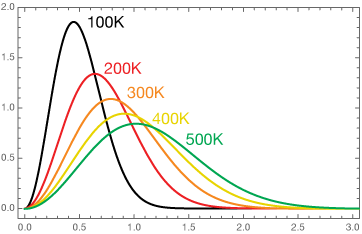
\includegraphics[width=0.8\textwidth]{MBGraph2.png}
        \caption{Maxwell-Boltzmann distribution of particles in energy levels}
    \end{figure}
\end{definition}
\begin{definition}[Change of Entropy for an Ideal Gas]
    The change in entropy of an ideal gas is:
    \begin{equation}
        \Delta S = s_2 - s_1 = k_B \ln\left(\frac{\Omega_2}{\Omega_1}\right) \\
    \end{equation}
    After some derivation, we have:
    \begin{equation}
        \Delta S = mR \left[ \ln\left(\frac{3}{2} \frac{T_2}{T_1}\right) + \ln\left(\frac{V_2}{V_1}\right) \right]
    \end{equation}
\end{definition}
\chapter{Heat Transfer}

\end{document}
